\documentclass[a4paper]{article}
\usepackage[utf8]{inputenc}
\usepackage{amsmath}
\usepackage{amssymb}
\usepackage{tikz}

\begin{document}

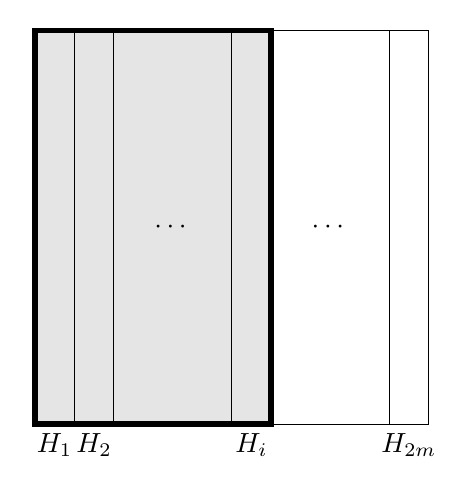
\begin{tikzpicture}
    % highlight and border
    \filldraw[gray!20] (0.0,0) rectangle (3,5);
    \draw[line width=2pt] (0,0) rectangle (3,5);
    \draw (0,0) rectangle (5,5);
    % separating lines
    \draw (0.5,0) -- (0.5,5);
    \draw (1.0,0) -- (1.0,5);
    \draw (2.5,0) -- (2.5,5);
    \draw (3.0,0) -- (3.0,5);
    \draw (4.5,0) -- (4.5,5);
    % text
    \node[anchor=north] at (0.25,0) {$H_1$};
    \node[anchor=north] at (0.75,0) {$H_2$};
    \node[anchor=north] at (2.75,0) {$H_i$};
    \node[anchor=north] at (4.75,0) {$H_{2m}$};
    \node at (1.75,2.5) {$\cdots$};
    \node at (3.75,2.5) {$\cdots$};
  \end{tikzpicture}

\end{document}